\documentclass[11pt]{article}
\usepackage[]{graphics}
\usepackage{natbib}
\usepackage[margin=2cm]{geometry}
\usepackage{rotating}
\usepackage{subfloat}
\usepackage{color}
\usepackage{outlines}
\usepackage{parskip}
\usepackage{pgfgantt}
\usepackage{appendix}
\usepackage{comment}
\usepackage{hyperref}
\usepackage{cleveref}
\usepackage{xcolor}
\usepackage{multirow}
\newcommand{\code}[1]{{\texttt{#1}}}

\setlength{\parindent}{2em}
\setlength{\parskip}{0.25em}

\title{Developing an Intelligent Train Booking Chatbot}
\author{Group 7 (AKOBot): Alexander Ferguson, Kaloyan Valchev and Omar Mostafa}


\begin{document}

\maketitle

\begin{abstract}
    
    Nowadays, a lot of train booking websites are available to the public to use. However, it can get difficult to book a journey with the best price possible since there are many websites to look at. This paper aims to document the design and development of an intelligent train booking chatbot to find the cheapest tickets for their journey, improve customer satisfaction and predict train delays. The chatbot is able to book tickets and predict delays but was not able to create a very accurate and reality-close prediction. 

\end{abstract}

\tableofcontents

\section{Introduction}
Businesses and other institutions nowadays rely on many forms of automation. It can range from automating tasks in software development environments such as automated tests to customer facing tasks such as answering customer queries. This project seeks to develop such a chatbot for booking train tickets and assess its success. Successful chatbots in this case would benefit many people as it fetches the cheapest tickets available and gives estimate times on train delays automatically which is more efficient than employing a human since it saves capital and time.



    \subsection{Background and Motivation}
    A chat bot is a computer system that allows a two way conversation, with only one user. The application usually consists of user interface where user can input requests and receive responses, database where the system stores data to learn from and a reasoning engine which serves as logical evaluation tool on which responses are generated. A chatbot provides easy access of information, saves time on monotonous tasks and reduces the need of employees dealing with common requests.


    In order to satisfy the module's requirements and courseworks, we have been tasked to create this chatbot to book train tickets, predict delays and provide good customer interaction. \citep{AI2020CW}

    \subsection{Aim and Objectives} 

    The aim of this project is to develop an intelligent chatbot that can help train commuters with various aspects of travelling by doing things such as helping book tickets and predicting train delays.

    The objectives are as follows:
    \begin{itemize}
        \item Providing good user experience (UX) with a good website user interface (UI)
        \item Creating a knowledge base/database
        \item Learning about and creating a Natural Language Processor (NLP) module
        \item Learning about reasoning engines and creating them
        \item Creating a predictive model for train delays
    \end{itemize}


    \subsection{Difficulties and Risks}

    We faced risks in developing the chatbot which include:

    \begin{itemize}
        \item \textbf{COVID-19 Situation}: It's a risk since it limits our face-to-face sessions as a group which can affect our teamwork. This however is not new experience to any of us, since we all have done a year in industry placement and are used to working from home and communicating over online platforms. However, it proved to be a big risk since one of the team members was living with infected members and this caused a disruption in their development work.
    
        \item \textbf{Other Module Deadlines}: Since other modules have deadlines in the same time frame, it forces members to shift focus away from this coursework and results in less work done. To mitigate this, we have planned for this by having a 2 week break from this coursework in order to focus on other modules, and after that all focus will be on this chatbot development.
    
        \item \textbf{Experience}: Since this is a module dealing with artificial intelligence topics such as NLP, predictive models, reasoning engines which none of us have worked on before, it poses as a risk to planning since we would most likely underestimate requirements or not be able to finish tasks on time. We try to mitigate this by using the documentation available and help from the module organizer's surgery sessions.
    \end{itemize}

    \subsection{Work Plan}

    This Gantt chart starts at e-vision week 14 (after 2/11/2020) because this is when our group was formed.


    The coloured bars represent times when the chatbot will not be worked due to reasons such as other courseworks from other modules.


    The dotted bars represent times when some work is being put into the chatbot, but with limited capacity as not all members of the group would be working on it at that time.


    \begin{figure}{Initial Project Gantt chart \label{pplan}}
    \begin{sideways}
    \newganttchartelement{voidbar}{
        voidbar/.style={
        draw=black,
        top color=black!25,
        bottom color=black!23
        }
    }
        \begin{ganttchart}[x unit=1.2cm, vgrid, title label font=\scriptsize,
            canvas/.style={draw=black, dotted},
            /pgfgantt/milestone left shift = .25,
            /pgfgantt/milestone right shift = -.25,
        ]{1}{13}
        \gantttitle{Project schedule shown for e-vision week numbers
     and semester week numbers}{13} \\
        \gantttitlelist{14,...,26}{1}\\
        \gantttitlelist{6,...,12}{1}
        \gantttitle{CB}{4}
        \gantttitle{1}{1}
        \gantttitle{2}{1}
        \\
    
    
    %the elements, bars and milestones, are identified as elem0, elem1, etc
    
        \ganttvoidbar{Working on Other Courseworks}{1}{2}     %elem0
        \ganttbar[bar/.append style={pattern=north west lines}]{}{3}{3} \\ %elem1
        \ganttbar{Research and Design}{3}{4} %elem2
        \ganttbar[bar/.append style={pattern=north west lines}]{}{3}{3}  \\ %elem3
    \ganttbar{Implementation}{4}{5}      %elem4
    \ganttvoidbar{}{5}{5}              %elem5
    \ganttbar[bar/.append style={pattern=north west lines}]{}{6}{6}   %elem6
    \ganttbar{}{7}{11} \\     %elem7
    \ganttmilestone{Outline Report Delivery}{5} \\ %elem8
    \ganttmilestone{Interim Report Delivery}{7} \\ %elem9
    \ganttbar{Testing}{7}{12}              \\  %elem10
    \ganttmilestone{Demo and Submission}{13}        %elem11
    
    
    \ganttlink{elem1}{elem3} \ganttlink{elem2}{elem4} \ganttlink{elem7}{elem8}
    \ganttlink{elem8}{elem9} \ganttlink{elem9}{elem10} \ganttlink{elem10}{elem11}
    \end{ganttchart}
    \end{sideways}
    \end{figure}
    \newpage

    \subsection{Team Development}
    This team will use the agile methodology since all 3 members of the group have used and practiced it before in their year in industry and due to this method's convenience in small-scale prototyping projects, it has been chosen as the method to follow in developing AKOBot. In order to track work to do and to be done, the team used Trello and held weekly Microsoft Teams meetings to discuss work done by each member and the difficulty of each ticket and the distribution of such work.

    The codebase is stored and maintained in a private repository on GitHub due to its ease of use and version control and most members used GitKraken in order to checkout the codebase and work on it on their local machines. The project codebase was edited and interpreted using JetBrains PyCharm and Microsoft Visual Studio Code.

    \subsection{Work Distribution}
    Each member has been given certain components of the coursework to work on and are as follows:

    \begin{table}[h]
    \begin{tabular}{lllll}
    \textbf{Name}               & \textbf{Contribution} & \textbf{Coursework Parts}                     &  &  \\
    \textit{Alexander Ferguson} & 33\%                  & NLP, Reasoning Engine and UI     improvements &  &  \\
    \textit{Kaloyan Valchev}    & 33\%                  & Predictive Model and UI     creation          &  &  \\
    \textit{Omar Mostafa}       & 33\%                  & Database and Report                           &  & 
    \end{tabular}
    \caption{A Table showing contributions of each team member}
    \label{tab:contribTable}
    \end{table}
    

\section{Related Work}
    \subsection{ELIZA}
    Although chatbots might seem like a relatively new concept, they have existed ever since the 1960s with ELIZA being one of the first. The paper about this chatbot was published in 1966 and is considered to be a rule-based chatbot. ELIZA tries to understand the input by parsing each word from left to right and gives it a rank based on importance by looking up the word in a dictionary of keywords. The word with the highest rank would then be used as the word to be pattern matched and so the appropriate response is given. ELIZA was mostly able to keep the conversation going even when it could not understand the input which made it special. \citep{ELIZA1966chatbot}

    \subsection{ALICE}
    ALICE, short for Artificial Linguistic Internet Computer Entity, was developed in 1995-2000 to make it easier for users to input answers for the chatbot to use. It was inspired by ELIZA but is different in many ways such as having a knowledge base and the lack of natural language processing since it uses AIML  (Artificial Intelligence Markup Language), a form of XML (Extensible Markup Language), to understand input. 

    The input given is taken and a depth first search is performed on the knowledge base using each word. When the response is found, it is stored and then the next word is searched again. This is done until there are no more words, in which then all the responses are combined. \citep{abushawar2015alice}

    \subsection{Customer Facing Chatbots}
    In recent years, automated chatbots have gained popularity and has been used to answer simple and frequently asked questions using the knowledge base which is updated by the company. The main reasons chatbots are being used more now is due to the financial benefits of not having to employ more workers to chat with the customer and the time saved since the information can be fetched by the chatbot quickly compared to a human employee. A downside for this is that the chatbot can sometimes not be able to answer all questions given by the customer, so humans have to intervene in such cases \citep{galert2018chatbot}.

    \subsection{Virtual Assistants}
    Virtual assistants have emerged during the last decade and represents a major step in the advancement of open-domain chatbots. Examples include Amazon's Alexa, Microsoft's Cortana, Google Assistant and Apple's Siri. They are able to answer multiple random questions or answer queries about real time situations such as a current day's weather using its cloud servers which receives these questions \citep{burbach2019hey}.

    On top of the functionalities mentioned they are also able to complete tasks such as playing songs, creating reminders in calendars, order groceries, etc.. This is all done through voice conversations by the user and the chatbot itself using its speakers, so it relies on its speech recognition capabilities much more than other chatbots. 

    It relies on advanced NLP and other artificial intelligence methods to figure out users' intent in a swift and accurate manner \citep{sri2020nlp}.


    \subsection{Travel Booking Chatbots}
    Looking at more related and specific examples to our project, \citep{lino2018travel} looked at developing a travel booking chatbot by booking car rentals, flights and hotel rooms at the same time. This was done using DiagFlow NLP which recognizes users' intent by training it using examples, and sending this information on to the webhook server where this chatbot backend resides in. This chatbot was successful due to the surveys and the fact that it was able to complete the its tasks while improving customers service with its layout.

    A more established example of such chatbots could be the Expedia chatbot \citep{expediaBot} which uses Facebook Messenger as its user interface to book trips. With examples of more companies using such companies, it shows the general shift of the travel booking industry towards a more automated one due to its speed and customer interaction.


\section{Design of the Chatbot}\label{sec:DesignMain}
This section aims to show the design planned out by the team before the implementation stage.

In terms of programming language, the considerations made mainly related to support available during labs, the available libraries and team experience with a language. As \code{Python} was the only lab-supported language for this assignment, it was the first language that was evaluated. The libraries available in \code{Python} seemed to meet the majority of the requirements and the team’s experience in this language was sufficient enough to justify using it.

    \subsection{Requirements Analysis}
    We have used a MoSCoW approach to pinpoint the most important sections of the project and have structured them as follows:

    \begin{itemize}
        \item  Must have:
        \begin{itemize}
            \item User interface where user input and response from the system will be displayed
            \item Input field for user to type their request
            \item Option to book a ticket
            \item Option to predict train delay
            \item Delay predicting engine
        \end{itemize}
    \end{itemize}
    \begin{itemize}
        \item Should have:
        \begin{itemize}
            \item Database to store train data for delay prediction
            \item Reasoning engine to understand user input and provide accurate response
            \item Web scraper to pull ticket from website with provided input from user
        \end{itemize}
    \end{itemize}
    \begin{itemize}
        \item Could have:
        \begin{itemize}
            \item Mobile web responsive UI
            \item Database to store previous conversations
            \item Option for speech-to-text and text-to-speech input from user
            \item Option to provide support (e.g. how to reach X train station)
        \end{itemize}
    \end{itemize}
    \begin{itemize}
        \item Won`t have:
        \begin{itemize}
            \item Open domain chat
            \item Mobile application
        \end{itemize}
    \end{itemize}

    \subsection{Conversation Flow}
    In order to understand how the bot will work as a whole, conversation flow example had to be generated which shows an example of how a typical conversation should go between the user and the system. The system would first greet the user and then ask them to specify if they want to book a ticket or get information about a delayed train.

    Figures \ref{fig:OldBookingFlow} and \ref{fig:predictFlow} show example of this.
 
    \subsection{The Architecture of the chatbot}
    The architecture was decided on a basis of rapid prototyping which means being able to implement parts of the system, testing it and integrating it as soon as possible. The reason for this is, since this is a quite new experience for us using such tools then we would want to quickly reflect our work in order to check if we are heading in the correct direction in terms of development or not. 
    
    Having a strict Model, View, Controller (MVC) would mean slowing down development work, so we implemented a "loose" MVC design in order to still have cohesion within the system but still be able to have freedom of quickly prototyping our chatbot.
    
    \begin{figure}[!ht]
        \centering
        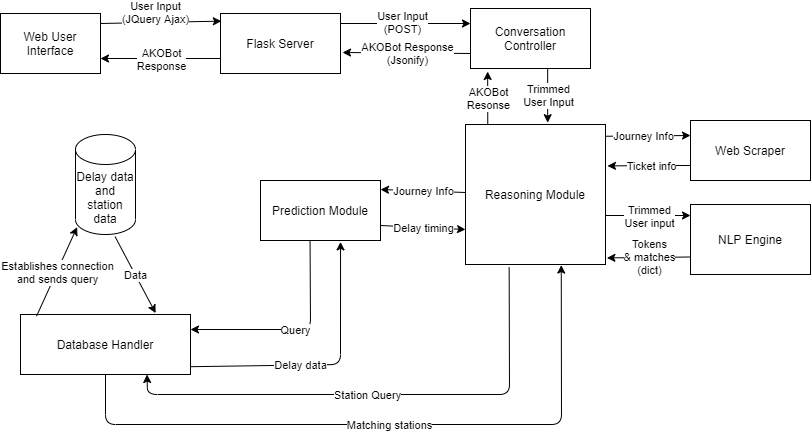
\includegraphics[width=0.85\textwidth]{ArchV1.png}
        \caption{A high level overview of the system design}
        \label{fig:ArchDesign}
    \end{figure}
    
        \subsubsection{Tags}
        The team planned on creating tags in the form of \code{TAG:XXX} or \code{REQ:XXX} which would help the system (mainly, the NLP and reasoning engine modules) in understanding the responses given by the user. These tags are interacted with in the UI, Conversation controller, NLP module and reasoning engine and will be discussed in the appropriate sections below.
        
        The idea of how this works is by binding the tags in the message text by adding it at the beginning of the message, where each component will clean the text to extract this info and preserve the original information. The tags are mainly created by the reasoning engine when a conversation is started, after establishing the intent of the user, with each question a tag is associated with it and tags the future response of the user. 
        
        For example, when the intention turns out to be booking a ticket, the reasoning engine produces a tag, \code{TAG:DEP}, because the question which it will ask is about the name of the station the user is going to depart from. So the user response to that question is tagged with tag mentioned previously, and passed to the components accordingly.

    \subsection{User Interface} 
    
    
        \subsubsection{Framework \& Tools Choice}
        The UI framework was decided upon based on the team’s previous experience. A console and web interface both were good options, but ultimately a web interface would be able to provide a richer, more interactive user experience.
    
        \code{Django} and \code{Flask} have both been used in previous modules to produce web interfaces with \code{Python}. \code{Django} did not seem a good fit due to its strict MVC approach, which could have slowed down development and not allow for quick prototyping of ideas. \code{Flask} is a simpler framework that deals just with rendering the front-end and seemed like it was well suited for performing that one task without imposing too many restrictions on the codebase.
    
        \subsubsection{Visual Design}
        The UI is a sleek, responsive web page which is designed using \code{HTML5} and \code{CSS}, rendered by \code{Flask} and has its contents and user facing functions implemented using \code{JavaScript} and \code{JQuery}. The aim was to provide a pleasant and modern design used in conversational UIs such as Facebook Messenger using curved message boxes, typing notifications and matching colours.
    
        AKOBot has its own custom logo, designed by a member of the team with heavy experience in UI design, which contains a train facing the user as an "O" which provides a custom pleasant look as seen in \cref{fig:AKObot_firstui}. The colours chosen match the university's official colours of blue and yellow.
        
        \begin{figure}[!ht]
            \centering
            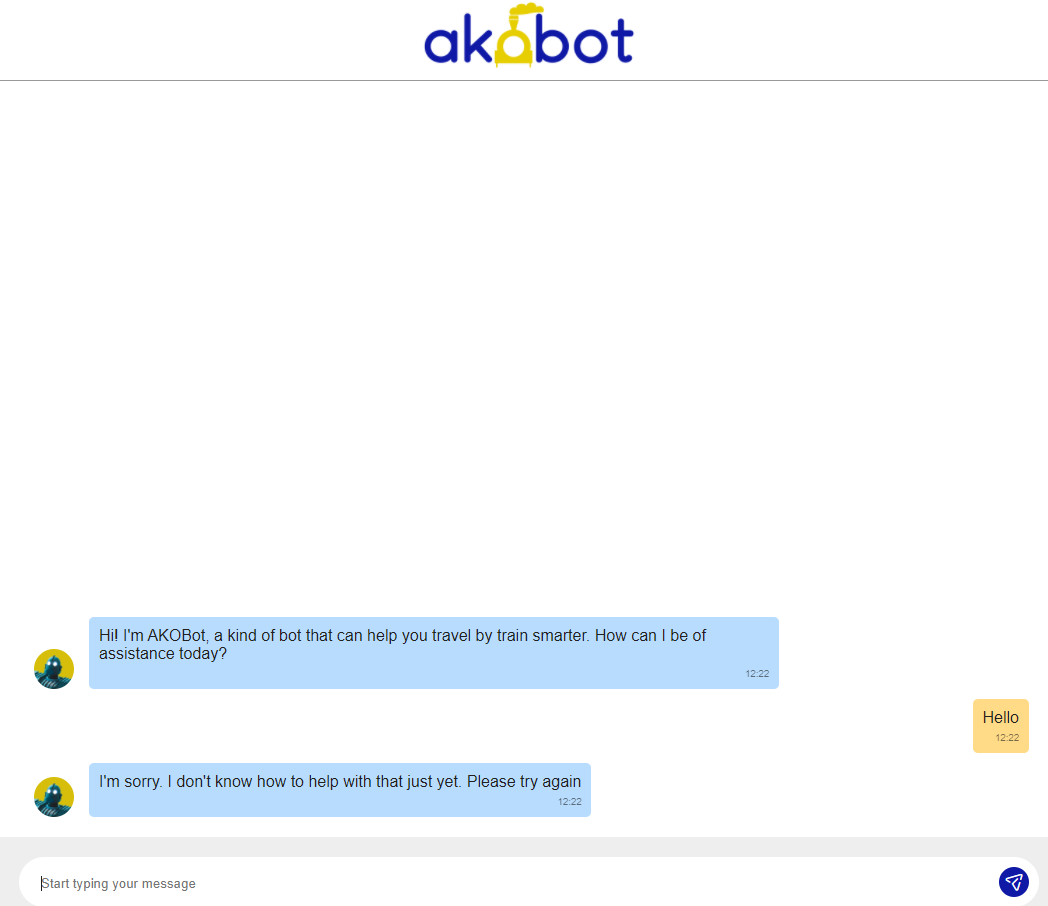
\includegraphics[width=0.75\textwidth]{AKObot_UI.PNG}
            \caption{A screenshot of the first implementation of the User Interface}
            \label{fig:AKObot_firstui}
        \end{figure}
        
        Another design choice was the inclusion of emojis, such as a thumbs up or down as shown in \cref{fig:sidebarAkobot}, as form of answering a question which helps in making the chatbot look more modern and sleek.
    
        \subsubsection{Software Design}\label{sec:UIDesignSD}
        The web interface is displayed by \code{HTML5} and its \code{CSS} files, and a \code{JavaScript} file is responsible for adding chat messages, updating the view of the UI and adding suggestion boxes which appear for the user to choose from. 
        
        The messages would be sent from the web interface through to the \code{Flask} server by making a \code{JQuery Ajax} call. The call to the backend is then sent by making a \code{POST} call which is requested by the conversation controller. When the response is received, the UI creates new \code{HTML} code to visually create the chat message box and add the bot's response to it along with suggestions if there are any, as used in \cref{fig:suggestloc}.
        
        \subsubsection{Tags}
         The user interface receives tags made by the reasoning engine inside the question sent by the user which is never shown to the user and assigns the replacement tag to the message response from the user to the question. These tags are mainly to help the NLP module and reasoning engine to understand the message which will be expanded upon in sections \ref{sec:NLPDesign} and \ref{sec:ReasoningDesign}, but the UI's purpose in this is to simply send tags back with certain replacements or sending it as is. A table of these replacements are shown in \cref{tab:UITagsReplacement}. One thing which is done to all other tags is changing its beginning from "{REQ:XXX}" to "{TAG:XXX}", to indicate that this message is from the user in response to the question referred to in the tag.
         
         For example, if the chatbot asks where the user is departing from and the user answers "Norwich", then the message to be passed will replace \code{\{REQ:DEP\}} which came from the reasoning engine, with "\code{\{FROM\} Norwich}.
         
\begin{table}[!ht]
\centering
\begin{tabular}{|l|l|l|}
\hline
\textbf{\begin{tabular}[c]{@{}l@{}}Original Tag\\ \{REQ:XXX\}\end{tabular}} & \textbf{\begin{tabular}[c]{@{}l@{}}Replacement Tag\\ \{TAG:XXX\}\end{tabular}} & \textbf{Representation} \\ \hline
\textit{DEP}                                                                & FROM*                                                                          & Departure Station       \\ \hline
\textit{ARR}                                                                & TO*                                                                            & Arrival Station         \\ \hline
\textit{DDT}                                                                & DAT                                                                            & Departure date/time     \\ \hline
\end{tabular}
\caption{A table of the tags that get replaced in the UI}
Note: Tags with the "*" sign simply have the curly brackets added to it only.
\label{tab:UITagsReplacement}
\end{table}
       

    \subsection{Conversation Controller}\label{sec:convcontDesign}
    This module is simply responsible for controlling how the messages are represented within the system and to the user. The controller receives input from the web UI by using \code{Flask}'s \code{request.form} to get the user's message and is able to control display of the UI by using \code{render\_template()} and directing the \code{Flask} server to display the webpage.
    
    It dictates how the chat is stored and passed around the system by storing the response given by the user and the bot, and starting up the reasoning engine to start processing the message given. It contains the opening message from AKOBot and an error handling message for whenever the browser encounters any kind of issue. When the reasoning engine is done with generating an answer, the conversation controller uses \code{pop\_message()} on the chat log which is modified by the reasoning engine and sends it back to the UI by using \code{JSONify} to send the answer in the form of \code{JSON}.
    
    The conversation controller also receives tags from the UI which is used to help the NLP module get a better understanding of a sentence passed to it. For example, it replaces "{TAG:DAT}" with "departing at" in order to help the NLP module process the sentence and provide an accurate result. The original tag is still preserved inside the message text when sent to the RE, it is only replaced in the copied message from the user in order to help the NLP. Replacements and their tags are shown in \cref{tab:DesignConvContTag}.
    
    \begin{table}[!ht]
    \centering
\begin{tabular}{|l|l|}
\hline
\textbf{Original Tag} & \textbf{Replacement text} \\ \hline
\textit{FROM}        & "departing from"     \\ \hline
\textit{TO}          & "arriving at"        \\ \hline
\textit{TAG:DAT}          & "departing at"       \\ \hline
\end{tabular}
\caption{A table of the tags and their replacements inside the conversation controller}
Note: The tags are surrounded by curly brackets
\label{tab:DesignConvContTag}
\end{table}
    
    \subsection{Natural Language Processor}\label{sec:NLPDesign}
    Both \code{NLTK} and \code{SpaCy} were considered. The team had a small amount of experience in \code{SpaCy} but very little with \code{NLTK}. \code{SpaCy} seemed to have better documentation, a more mature development ecosystem and free online tutorials on how to utilize it. This led to the conclusion that the \code{SpaCy} would be used as the NLP engine for the application. The \code{SpaCy} library is very straight forward, accompanied with quality documentation which promises results with little effort.
    
    
    Our NLP module is mainly used by the reasoning engine when it first stumbles upon a sentence which it has not yet understood. The reasoning engine calls the NLP module's \code{process()} which uses \code{SpaCy}'s default text processing function. It uses an already trained English pipeline model called \code{en\_core\_web\_sm} which was created by \code{Explosion.ai} and was easily integrated into the module. 
    
        \subsubsection{User Intention \& Information Extraction}
        The first task for the module is to identify if it is to perform one of the 2 main tasks:
    
        \begin{itemize}
            \item 'book' - The user wants to book a ticket
            \item 'delay' - The user wants a delay prediction for their journey
        \end{itemize}
    
        
        Deriving the intention of the user is a difficult task to do since we would have to consider the unpredictable behaviour of humans through the user's input. So the team had to plan a mechanism or strategy in order to accurately understand the user's intention and act upon those intentions.
        
        The mechanism follows:
        \begin{itemize}
            \item Tokenizing the input using \code{SpaCy}.
            \item Lemmatization of certain phrases
            \item Using Part-Of-Speech (POS) tagging to tag the tokens.
            \item Dependency Parsing 
            \item Pattern matching the tokens with \code{SpaCy}'s own vocab.
            \item Pattern matching the tokens with our custom token dictionary of phrases and intention (see \cref{tab:DesignTokenDict}).
        \end{itemize}
        
        
        The NLP module first removes the tags before being passed to \code{SpaCy}, then the input is tokenized and a \code{SpaCy.Doc} variable is returned which contains all the information from its analysis of the sentence. Once this is done a range of features such as Lemmatization of phrases is used so that words such as "book" can be derived from "booking" which means less phrases entered by us. POS is then performed in order to identify the features of each token i.e. identifying verbs, proper nouns, etc. POS is very helpful in easily identifying entities such as date and time which we would then use in the future.
        
        Dependency parsing was used in order to know which words have a dependency on previous words in the sentence, for example "London Liverpool Street" are 3 words but they would not make sense if they were separated or they weren't noted to have dependency on each other. Pattern matching is then done, using \code{SpaCy.Matcher}, against \code{SpaCy}'s vocab dictionary and our own dictionary (see \cref{tab:DesignTokenDict}) added to it which contains the most common phrases which we thought of when performing the 2 main tasks.
        
        The team had to take careful consideration on what phrases were most likely to be used when providing information or stating which task the user wants to use. 
        
    
    \begin{table}[!ht]
\centering
\begin{tabular}{|l|l|}
\hline
\textbf{Key}       & \textbf{Intention}         \\ \hline
\textit{book}      & Book a ticket              \\ \hline
\textit{delay}     & Get delay prediction       \\ \hline
\textit{yes}       & positive response/agree    \\ \hline
\textit{no}        & negative response/disagree \\ \hline
\textit{depart}    & departure station          \\ \hline
\textit{dep\_date} & departure date and time    \\ \hline
\textit{dep\_delay} & Train delay duration       \\ \hline
\end{tabular}
\caption{A table of our initial token dictionary and its intentions}
\label{tab:DesignTokenDict}
\end{table}

        \subsubsection{Tags}
        The tag replacements mentioned in \cref{sec:convcontDesign} and referenced in \cref{tab:DesignConvContTag} are mainly done in order to help with our basic NLP pipeline model in identifying station names and dates/times. In the event that the user supplies "Departing from Norwich" when answering a question about the departure station, the conversation controller will make this sentence into "departing from departing from Norwich", the NLP will still be able to identify the station or other entities correctly.

        \subsubsection{Date and Time}
        When the dates and times are identified, we would then have to transform the token into a variable which is easily understood by the system. 
        
        For this purpose, we decided to use \code{dateparser} which would derive the day, month and other aspects of date and time accurately in order to be used by other components with data integrity i.e. correct date and time. This package is also able to process phrases such as "today" or "tomorrow" which brings variety in what kind of responses AKOBot will accept.


    \subsection{Database}\label{sec:DesignDB}
    The database is essential to AKOBot in order to function correctly and provide a smart storage solution for the amount of data that needed to be stored. 

    The database will contain two tables, \code{Stations} and \code{TrainingData}, which will contain each station's 3 letter code and train delay data sets from the national rail, respectively. It was decided to use \code{SQLite} due to its compactness and ease of integration since it is an included library with \code{python3} and it would be included in the version controlled repository, meaning any mistakes in the database will be highlighted and reviewed before merging with a clean version of the database.
    
    The requests to the database and its responses will be handled by a database handler module, responsible for establishing a connection between the project and the database and sending the queries to the database. The database handler would then receive the data in tuples and would send it to the components that requested the data.
    
    \subsection{Web Scraper}
    The web scraper is responsible for finding the cheapest ticket possible according to the information provided by the user. The module receives a dictionary full of the information of the journey and accordingly constructs the URL based on \textit{nationalrail.co.uk}, which is the national rail network's official website for booking tickets. Once the URL is available, the link is then opened using \code{urlopen} from the \code{requests} package and the \code{HTML} is stored and then parsed by \code{BeautifulSoup}. 
    
    The cheapest ticket is found by searching for the special tag specified by the website for the cheapest price which is \code{class:fare has-cheapest}. The price is then taken along with the information specified in this ticket's script contents on the website and turned into \code{JSON} which is passed back to the reasoning module along with its URL.


    \subsection{Reasoning Engine}\label{sec:ReasoningDesign}
    The reasoning engine (RE) functions as "the brain" of the chatbot by triggering the NLP module and other components of the chatbot according to the information presented at hand. \code{Experta} was chosen as the reasoning engine to use due to its reasonable documentation and popularity compared to other engines.
    
        \subsubsection{\code{Experta} Syntax}
        The RE functions by having a set of rules and facts on which it operates upon. The facts are declared by the module using \code{declare()} and is modified using \code{modify()}. Whenever a fact is changed or added, \code{Experta} checks all the facts and rules exist and decides if there are any rules which match the stated facts and triggers it accordingly using the functions which have those rules associated with it.
        
        The rules follow a condition-action pair-like mechanism where the left-hand side of the rules are the conditions on which the rule should be executed and the right hand side is where the set of actions preside on which it is executed when the rule is executed. \code{\@Rule} is used to specify the conditions or facts to match, after-which it will execute when conditions are met.
        
        In the event more than one rule have their conditions met, \code{salience} is attributed to each rule in order to prioritize which rule is to be executed.
        
        \subsubsection{Usage}\label{sec:REUsageDesign}
        The \code{Experta} engine has to be reset everytime we run our module, so we had to create a knowledge dictionary exists which contains all the facts. The reasoning engine is first initialized using \code{\@DefFacts} and is associated to \code{\_initial\_action()} which acts as a generator, which assigns all the facts to the engine from the dictionary. If the "action" or "complete" fact keys are not found, then they are assigned to "chat" and false, respectively to start the conversation with the greeting message. \code{direct\_to\_correct\_action()} is called since it meets the conditions and has the highest \code{salience} in the system (100), it is used to determine what task the user wants the chatbot to do (booking a ticket or delay prediction). 
        
        When the user's intention is known, the chatbot is initialized with a string of 2 letter codes to represent the chatbot's progress towards finishing the task. Booking and delay prediction both have their own progress codes as shown in \cref{tab:InitProgCode}. Both booking and delay prediction tasks use the same progress codes except \code{dd} which used in delay prediction only. The codes are put in a string in the format \code{"dl\_dt\_al"} and each code is removed when the correlating action is performed. This helps the reasoning engine identify when all the information needed from the user is available.
        
\begin{table}[!ht]
\centering
\begin{tabular}{|l|l|l|}
\hline
\textbf{Task Usage}                                                                     & \textbf{Progress Code} & \textbf{Value}                 \\ \hline
\multirow{3}{*}{\begin{tabular}[c]{@{}l@{}}booking and delay\\ prediction\end{tabular}} & \textit{dl}            & Departure station info given   \\ \cline{2-3} 
                                                                                        & \textit{dt}            & Departure date/time info given \\ \cline{2-3} 
                                                                                        & \textit{al}            & Arrival station info given     \\ \hline
delay                                                                                   & \textit{dd}                     & Duration of delay time given   \\ \hline
\end{tabular}
\caption{A table of the progress codes used for booking and delay prediction}
\label{tab:InitProgCode}
\end{table}

        It's worth noting that each rule has a method associated with it which is executed when certain conditions are met. For example, when the booking is not yet complete, then we would want the RE to ask the correct questions in order to gather all information. \code{booking\_not\_complete()} has rules which suggest not all information for ticket booking is available, where it will match those conditions and execute it.
        
        \subsubsection{Booking a ticket}\label{sec:REBookingTicket}
        As suggested in section \cref{sec:REUsageDesign}, once the user specifies that they want to book a ticket, the \code{booking\_not\_complete()} method is executed where it processes the user input and checks if it has any of the information needed such as arrival and departure station. The main conversation flow (as discussed in \cref{sec:convcontDesign}) is to ask the user where they are departing from and associating that message with the matching tag from \cref{tab:TagDesignRE}, in which case is "{REQ:DEP}". The RE then receives the user's message with our tag now called "{TAG:DEP}" which has been replaced in the UI, suggesting that the user message is in response to a question about what the departure station name is.
        
        When a departure station is found for example, \code{get\_dep\_arr\_station()} then modifies the "depart" fact to include the station name. The \code{booking\_not\_complete()} method checks at the end if the progress codes still exist i.e. not all information is available, and then modifies the fact "extra\_info\_req" to \code{True}. In this case, the \code{Experta} engine is then run with these new facts and identifies the highest salience rule with matching conditions. The matching rule at that point would be the  \code{ask\_for\_departure\_date()} method which then adds the question to ask for the departure date/time and modifies the fact "extra\_info\_requested".
        
        When the all the information needed is gathered and the progress code is empty, the facts will match the rules on \code{generate\_message()} which modifies the "final\_message\_sent" fact to \code{True} and ask the user to verify the information for the ticket. 
        
        Once the RE has all the information needed to search for the cheapest ticket, \code{generate\_ticket()} will match the conditions and be executed, which triggers the web scraper and receives the ticket information accordingly. The user is then informed of the price of the ticket and given an option to visit the URL to book the ticket, and the ending message is sent and at that point the \code{Experta} engine will be halted.
        
        \subsubsection{Delay prediction}
        Delay prediction uses \code{delay\_not\_complete()} in order to gather information about delay predictions. It follows the same steps as in \cref{sec:REBookingTicket} to gather information about the departure and arrival station, and departure date/time while using corresponding facts in \cref{tab:REFacts}. 
        
        It has an extra step where it needs to ask about the amount of time the train is delayed by to the user in which case, \code{Experta} will identify that \code{delay\_time()} needs to be called to ask the user. The user response will then be sent to the RE, which will figure out it's the delay duration using tags in \cref{tab:TagDesignRE}, and the RE will set the "departure\_delay" fact with the duration delay in seconds and the progress code will be empty. This causes \code{delay\_not\_complete()} to set the "complete" fact as true which will trigger \code{predict\_delay()} to be executed which will pass this information to the predictive model module and receive its predicted delay. A message is then sent informing the user of the predicted delay and will then end the conversation with an ending message.
        
        \begin{table}[!ht]
\centering
\begin{tabular}{|l|l|}
\hline
\textbf{Tag} & \textbf{Intention}  \\ \hline
\textit{DEP} & Departure Station   \\ \hline
\textit{ARR} & Arrival Station     \\ \hline
\textit{DDT} & Departure date/time \\ \hline
\textit{DDL} & Delay duration      \\ \hline
\textit{DLY} & Delay departure date/time      \\ \hline
\end{tabular}
\caption{A table of the tags that are sent and received across the system}
\label{tab:TagDesignRE}
\end{table}
    
    
    
        \subsubsection{Station Matcher}
        A station matcher was implemented in order to improve user experience for whenever a misspelled station name is typed in which is done using the reasoning engine's \code{get\_similarity()} function. This makes the chatbot smarter by not having such a restrictive input of station names and instead be able to help the user find the correct station. This also includes being able to input the 3 letter code of the station and reasoning engine will take it and derive the station name from it by querying the database. It's called in \code{get\_dep\_arr\_station()} which finds station names.
        
        % The \code is split up in order for the text to not go beyond the paragraph margins.
        The station matcher \code{SequenceMatcher} which essentially compares two strings by utilizing the \code{longest} \code{contiguous matching subsequence} (LCS) algorithm, which finds the longest match similar between both words and uses other methods to output a ratio (float between 0 and 1) representing the similarity. We retrieve all the stations in our database and compare it with our provided station name and multiply all the ratios by 100 and store it in a list to represent the most similar stations suggested by the \code{SequenceMatcher}.
        
        Each ratio is increased if it meets certain conditions which we have set, such as if the user input station name is at the beginning of the database-retrieved station name or is inside it e.g. User inputs "Birmingham", which highly refers to "Birmingham New Street" or "Birmingham Snow Hill". We found the best ratio increase to be 25 after multiple iterations with phrases such as "Liverpool" and "Birmingham".
        
        The 3 stations with the highest ratios are then chosen to be suggested to the user.

    \subsection{Predictive Model}
    AKOBot was required to predict delays for the Norwich - London Liverpool Street line when asked by a commuter whose train has not yet departed their station. So we created a machine learning predictive model which was trained using the data set mentioned in \cref{sec:DesignDB} which provides the required input for the model to learn from.
        
        \subsubsection{Data Preparation}\label{sec:DesignModelPrep}
        The data set used contains all the daily journeys between 2017-2019 and provides information such as the planned and actual arrival and departure times of each train at each station on that line.

        The information mentioned above was to be taken as a query to the database and several checks were conducted to make sure the data being passed to the model was not skewed such as making sure the times for stations were not empty/null.

        \subsubsection{Parameters/Input}
        With the data prepared to be used by our module, parameters had to be defined to determine how our models were to learn from the data that was being consumed. 
    
        The datasets from the national rail was analyzed to identify the best factors to increase accuracy of the model. The factors that were identified and extracted from the datasets are shown in \cref{tab:ModelInput}.

\begin{table}[!ht]
\centering
\begin{tabular}{|c|l|}
\hline
\textbf{Input}                                                & \textbf{Value}  \\ \hline
\textit{Day of the week}                                      & 0 to 6          \\ \hline
\textit{Rush hour}                                            & 1 or 0          \\ \hline
\textit{Weekend or Weekday}                                   & 1 or 0          \\ \hline
\textit{Segment of the day}                                   & 1 to 4          \\ \hline
\textit{Difference between planned and actual departure time} & Time in seconds \\ \hline
\end{tabular}
\caption{A table of the inputs and its values}
\label{tab:ModelInput}
\end{table}
    
        "Day of the week" has 0 as a Monday with increments through the week to 6 as a Sunday. The "Rush hour" input value being 1 means that it's during rush hour, "Weekend or Weekday" having 1 as an indicator that it is a weekday. "Segment of the day" is divided into 4 sections, Morning, Midday, Evening and Night,  with 5am being the starting point for Morning and the difference between each section is 5 hours. For example, a train at 2 pm is considered Midday which means the value is 2. The "difference for planned and actual departure time" is represented as seconds by subtracting these dates and times as seconds starting from 1/1/1900.
    
        Some of these inputs were chosen due to its relevance in detecting delay such as the rush hour \citep{NetworkRail}.
    
        Also, the main reason we choose to give so many inputs is to allow the model to learn about the factors which contribute to a delayed train and its severity. The best way to do so is to point the model to the properties of each journey and delay, which would make the model smarter.

        \subsubsection{K-Nearest Neighbour Model for Regression}
        Short for KNN, this model is a supervised machine learning model which was established as the go-to model for our rapid prototyping environment since we wanted to create models quickly and test them. This model was used as an indicator for the minimal function of the predictive model module as we wanted to quickly implement a working model. 
    
        This supervised machine learning model needed labelled data in order to function correctly, which is why the work in \cref{sec:DesignModelPrep} was necessary to do.
    
        In order to make sure of the accuracy of the model, it was decided to split the data 80\% for training the model and 20\% for testing the model. 



\section{Implementation}
As we started implementing the proposed design shown in \cref{sec:DesignMain}, we stumbled upon issues which required changes in certain components. After these issues were solved, we started improving the system overall and added support for more features in the chatbot which required even more changes in the components. This section aims to document all of these changes and the steps taken to solve the issues.

Some of the changes included adding support for the user to specify how many adults and children will be booking as well as asking if they would like a return ticket.

    \subsection{User Interface}
    The user interface has been improved upon heavily in visual and functional terms which will be documented in this section.

    The font used in the UI had been changed to a custom, non-standard one from \textit{Google Fonts} called \code{Space Grotesk} which offers a unique and appealing look to the user instead of the usual common fonts used by most chatbots.

    A starting/greeting page had also been designed in order to improve the customer experience and give an initial impression on the user on what is to come from using AKOBot. The page greets the user and contains a retro video on the national rail playing in the background without audio, which offers aesthetic and friendly feel to the user as shown in \cref{fig:akobotintro}.


\begin{figure}[!ht]
    \centering
    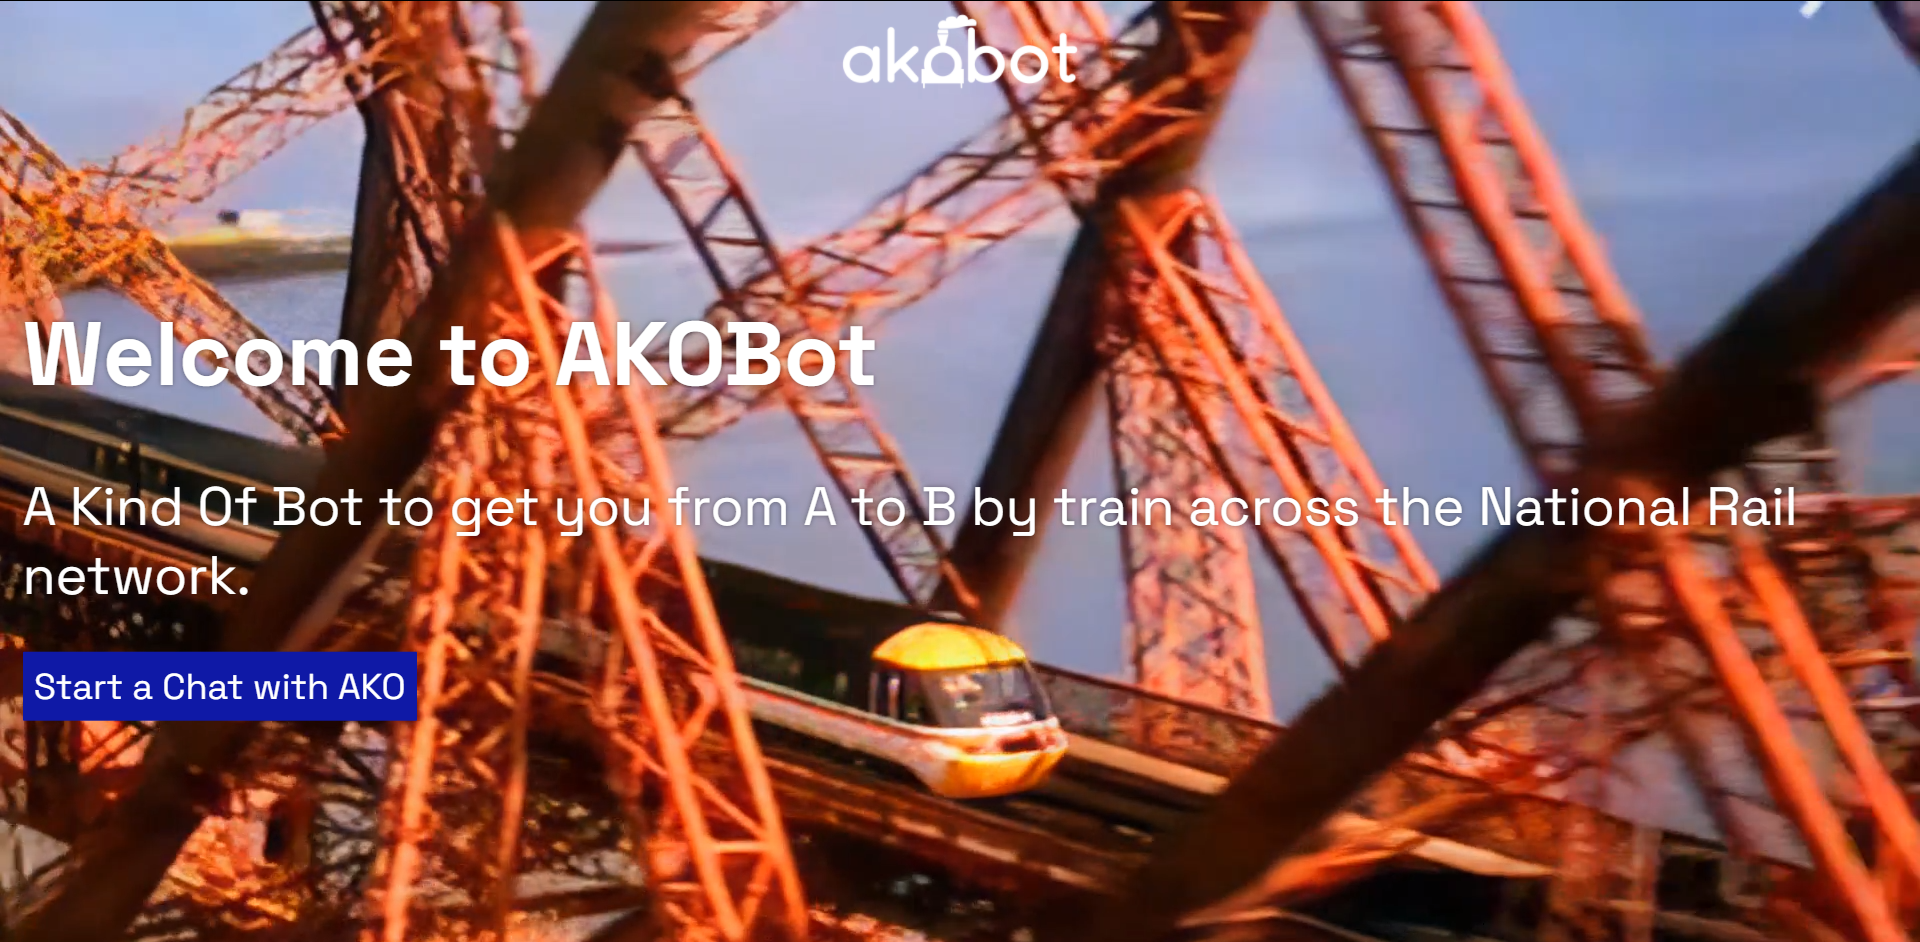
\includegraphics[width=.75\textwidth]{AkobotUIIntro1.png}
    \caption{A screenshot of the AKOBot greeting page}
    \label{fig:akobotintro}
\end{figure}

    A sidebar had also been designed and implemented in order to show the user the main tasks that AKOBot can perform, including a custom designed ticket, discussed further in \cref{sec:ticketDesignImp}, which is populated with information every time the user answers corresponding questions or provides it from the beginning as shown in \cref{fig:sidebarAkobot}.
        
        
        

    
        \subsubsection{Mobile View/Portability}
        Since we already chose a web user interface, it's possible for all kinds of platforms to support this chatbot as long as it is able to support web browsing. We were focused at first on designing the user interface for the desktop platform as a priority and after we created a minimum viable product, we investigated mobile views using our chatbot since some components of the UI might be unusable on the mobile view due to the smaller screen. We decided to have the sidebar removed for the mobile view only because it would have taken precious space on the already small screen and made the experience unbearable. An example of the chatbot working on mobile phones can be seen on \cref{fig:mobileAKOBotPic}.
        
\begin{figure}[!ht]
    \centering
    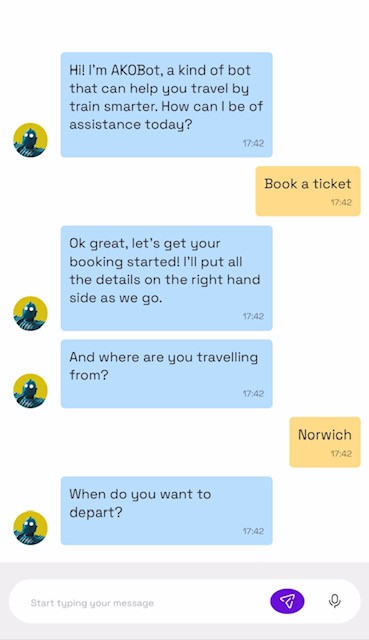
\includegraphics{MobileViewAkobot.jpg}
    \caption{A screenshot of AKOBot working on a mobile phone}
    \label{fig:mobileAKOBotPic}
\end{figure}

        \subsubsection{Text-To-Speech}\label{sec:texttospeech}
        The web UI automatically reads the messages sent by the bot by including \textit{Microsoft's} \code{SpeechSDK} in our \code{HTML} file and calling \code{speakSsmlAsync()} through \code{JavaScript}.
        
        \subsubsection{Speech-To-Text}
        Using the same package used in \cref{sec:texttospeech}, The user has the ability to press a microphone icon and proceed to talk to AKOBot in response to one of its questions. The \code{JavaScript} file uses the package and types in the response in the message box.

        \subsubsection{Geo-Location}
        
        \begin{figure}[!ht]
    \centering
    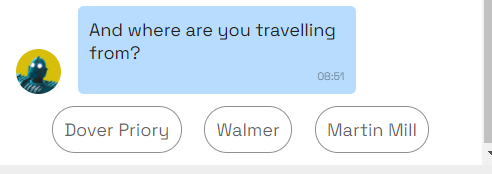
\includegraphics{LocationSuggestions.png}
    \caption{An example of location suggestions provided by AKOBot}
    \label{fig:suggestloc}
\end{figure}
        
        Using \code{HTML5}'s Geo-location API, we are able to retrieve the user's browser information regarding the location through the user's longitude and latitude. This information is fetched as soon as the user allows the website access to this permission and once it is granted, the UI waits until the chatbot sends a request asking for the departure station.

        If the user does not allow access, the chatbot asks where they would like to departure from, as usual. However, if access is allowed then the latitude and longitude is taken and given to \code{transportapi.com} by constructing the URL to include these coordinates. This retrieves the nearest train stations to the coordinates and is performed by making a \code{JQuery Ajax} call to the \code{Flask} server which then makes a \code{GET} request to \code{transportapi.com} and retrieving the closest stations. The 3 closest stations are then put as suggestions which can be chosen when the UI asks the user where they are departing from, as shown in \cref{fig:suggestloc}.
        
        
        
        \subsubsection{Tags}
        An extra tag, "{REQ:RTD}", was added to be replaced by the UI with "{TAG:RAT}" which is used for Returning date/time since we added support for return tickets. 
        
        \subsubsection{Ticket}\label{sec:ticketDesignImp}
        It was decided to create a ticket that would be updated on the user's view whenever any new information is entered in order to boost UX. The ticket visual design, based on the national rail's ticket design, offers a chance for the AKOBot to be clear to the user on the accuracy of the information being used/provided which would give the user confidence in the chatbot.
        
        The ticket is solely created using \code{CSS} in addition to the AKOBot logo in the background and since the national rail ticket is familiar to most users, it offers a welcoming experience and look as shown in \cref{fig:TicketView}. 
        
        \begin{figure}[!ht]
            \centering
            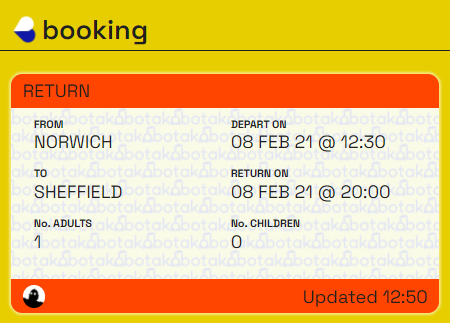
\includegraphics{TicketView.png}
            \caption{A screenshot of the ticket design in the UI}
            \label{fig:TicketView}
        \end{figure}
        
        The ticket uses the tags used by the system and additional tags solely for the ticket view to be updated. A list of those tags used to update the ticket's view on the UI is shown in \cref{tab:TicketTags}.
        
        \begin{table}[!ht]
\centering
\begin{tabular}{|l|l|}
\hline
\textbf{Tag} & \textbf{Representation} \\ \hline
\textit{DEP} & Departure station       \\ \hline
\textit{ARR} & Arrival station         \\ \hline
\textit{RET} & Single or Return        \\ \hline
\textit{ADT} & Number of adults        \\ \hline
\textit{CHD} & Number of children      \\ \hline
\textit{DTM*} & Departure date/time     \\ \hline
\textit{RTM*} & Return date/time        \\ \hline
\end{tabular}
\caption{A Table of the tags used to update the ticket's view in the UI}
Note: Tags with "*" mean they are solely created by the reasoning engine for the ticket view only and is not used anywhere else in the system.
\label{tab:TicketTags}
\end{table}

\newpage

    \subsection{Conversation Flow}
    Given there's support for return tickets, number of children and adults, the conversation flow changes since more questions need to be asked and information needs to be gathered. The new conversation flow for booking tickets is seen in \cref{fig:newbookingflow}.
    
    \begin{figure}[!ht]
        \centering
        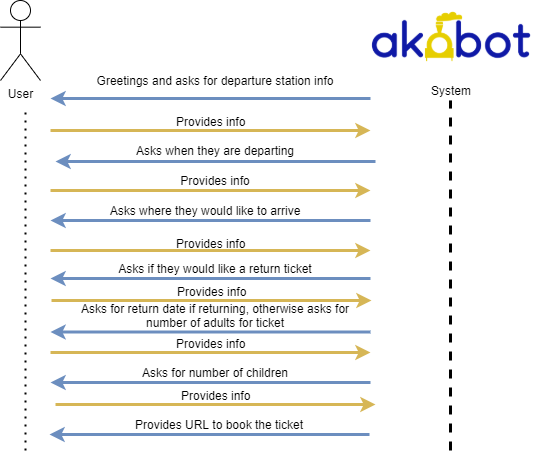
\includegraphics[width=0.75\textwidth]{NewBookingFlow.png}
        \caption{The new ticket booking conversation flow}
        \label{fig:newbookingflow}
    \end{figure}


    \subsection{Conversation Controller}
    
    The conversation controller was modified in order to replace an extra tag created for return tickets by replacing the system created "{TAG:RET}" with "returning at" in order to help the NLP module process the sentence and provide an accurate result. The full list of the tags and their replacements are in \cref{tab:ConvContImpTag}.
    \begin{table}[!ht]
    \centering
\begin{tabular}{|l|l|}
\hline
\textbf{Original Tag} & \textbf{Replacement} \\ \hline
\textit{FROM*}        & "departing from"     \\ \hline
\textit{TO*}          & "arriving at"        \\ \hline
\textit{DAT}          & "departing at"       \\ \hline
\textit{RAT}          & "returning at"       \\ \hline
\end{tabular}
\label{tab:ConvContImpTag}
\caption{A final table of the tags that get replaced in the conversation controller}
Note: Tags with "*" only have curly brackets around them, with no "TAG:" at the beginning of it.
\end{table}

    \subsection{Natural Language Processor}
    The initial token dictionary in \cref{tab:DesignTokenDict} was broken down and appended at the same time to accommodate for return journeys and specifying adult and children in bookings. The first dictionary contains simple phrases for each intention as shown in \cref{tab:SimpleTokenNLP}.
    
    \begin{table}[!ht]
\centering
\begin{tabular}{|l|l|}
\hline
\textbf{Token}      & \textbf{Intention}         \\ \hline
\textit{book}       & Booking a ticket           \\ \hline
\textit{delay}      & Delay Prediction           \\ \hline
\textit{yes}        & Positive response/agree    \\ \hline
\textit{no}         & Negative response/disagree \\ \hline
\textit{dep\_delay} & Train delay duration       \\ \hline
\textit{return*}     & Return ticket              \\ \hline
\textit{single*}     & One-way ticket             \\ \hline
\textit{num\_adults*} & Number of adults for booking       \\ \hline
\textit{num\_children*} & Number of children for booking       \\ \hline
\end{tabular}
\caption{A table of the simple tokens with their intentions}
Note: Tokens with "*" are the newly added tokens to support our newer features.
\label{tab:SimpleTokenNLP}
\end{table}
    
    
    The other dictionary is a multi dictionary, as shown in \cref{tab:ComplexTokenNLP}, has multiple for processing the various types of date and time entering and identifying station names when typed correctly which speeds up the process of answering the user quickly instead of using the station matcher from the RE. This solution helps the chatbot identify dates and times easily when using for example dashes instead of slashes in dates.
    
    \begin{table}[!ht]
\centering
\begin{tabular}{|l|l|}
\hline
\textbf{Token}     & \textbf{Intention}  \\ \hline
\textit{depart}    & Departure station   \\ \hline
\textit{arrive}    & Arrival station     \\ \hline
\textit{dep\_date} & Departure date/time \\ \hline
\textit{ret\_date} & Return date/time    \\ \hline
\textit{dly\_date} & Delay date/time     \\ \hline
\end{tabular}
\caption{A table of the complex tokens with their intentions}
\label{tab:ComplexTokenNLP}
\end{table}

    \subsection{Web Scraper}
    Since we added support for specifying adults and children, we had to change which website to use, because \textit{nationarail.co.uk} does not offer an option for specifying adults and children to be booked for the ticket. This also brings up a tougher problem because other websites usually have more \code{JavaScript} elements, meaning our design would not work, given the packages used can not handle these web pages correctly.

        \subsubsection{Website Change}
        We chose \textbf{chilternrailways.co.uk} because it was one of the few websites that allowed us to include the amount of adults and children in the URL which was being constructed.

        \subsubsection{Scraping the webpage}
        With this new website, \code{JavaScript} elements are now expected and could not be easily opened. So the team resorted to using \code{selenium} and \code{webdriver\_manager} to open the URL using a minimal headless instance of the \code{Mozilla Firefox} web browser which is installed on the user's side in order to open the \textit{chilternrailways.co.uk} website and scrape it. This is done using \code{webdriver\_manager.firefox}'s \code{GeckoDriverManager} which acts as a proxy between FireFox (which is a Gecko based browser) and the chatbot.
        
        Once the page has been scraped, the tag \code{"class:} \code{basket-summary\_\_total--value"} is used to identify the cheapest tickets and is then returned to the reasoning engine with the URL and ticket info including the price.



    \subsection{Reasoning Engine}
    The reasoning engine was modified in a few ways to welcome the new changes for supporting return tickets and more. Validation was added in order to combat the chatbot not being able to answer questions when presented with an undefined situation such as having the same station for the arrival and departure station.
    
        \begin{table}[!ht]
\centering
\begin{tabular}{|l|l|}
\hline
\textbf{Tag}  & \textbf{Intention}        \\ \hline
\textit{DEP}  & Departure station         \\ \hline
\textit{ARR}  & Arrival station           \\ \hline
\textit{DDT}  & Departure date/time       \\ \hline
\textit{DDL}  & Delay duration            \\ \hline
\textit{DLY}  & Delay Departure date/time \\ \hline
\textit{RET*} & Single or return ticket   \\ \hline
\textit{RTD*} & Return date/time          \\ \hline
\textit{ADT*} & Number of adults          \\ \hline
\textit{CHD*} & Number of children        \\ \hline
\end{tabular}
\caption{A final table of the tags which help the RE understanding}
\label{tab:FinalTagsRE}
\end{table}
    
    The RE has new rules and facts, as shown in \cref{tab:REFacts}, added to it in order to carry out these kinds of validation and add more questions to be asked by the RE to complete the booking procedure since we now ask for return tickets and number of children and adults. This also means adding newer tags as shown in \cref{tab:FinalTagsRE} and adding more progress codes specifically for the booking procedure as seen in \cref{tab:ProgCodeBook}.
    
    

    
    \begin{table}[!ht]
\centering
\begin{tabular}{|l|l|}
\hline
\textbf{Progress Code} & \textbf{Value}                         \\ \hline
\textit{dl}            & Departure station info given           \\ \hline
\textit{dt}            & Departure date/time info given         \\ \hline
\textit{al}            & Arrival station info given             \\ \hline
\textit{rt*}           & Return date/time info given            \\ \hline
\textit{rs*}           & Return ticket intention is known       \\ \hline
\textit{na*}           & Number of adults for ticket is known   \\ \hline
\textit{nc*}           & Number of children for ticket is known \\ \hline
\end{tabular}
\caption{A table of the progress codes for booking a ticket
Note: Those with "*" have been added during the implementation stage}
\label{tab:ProgCodeBook}
\end{table}

    \subsection{Predictive Model}
    Since the members of the team never had any experience machine learning libraries, a popular library with great documentation and easy-to-use functionality was needed, making \code{Sci-Kit Learn} the best option to go with. 
    
    Testing multiple training and testing data splits, the team has found that 70\%/30\%  ratio corresponding has produced best results. 
    
        \subsubsection{Models Used}
        Initially, KNN as regression was first implemented as designed and benchmarked the completion of the first complete version of AKOBot. As development went on, more models were added and tested which include:
        
        \begin{itemize}
            \item Support Vector Machine (SVM) as regression
            \item Random-Forest (RF) as classifier
            \item Multi-Layer Perceptron (MLP) as regression
            \item Multi-Layer Perceptron (MLP) as classifier
            \item 1 Nearest Neighbour (1NN)
        \end{itemize}
        
        After evaluating the models, we decided to use Random-Forest as the prime model delay predictions which will be discussed further in \cref{sec:evalmodel}.
        
        \subsubsection{Model Implementation}
        Since the models used were built at run-time, a decision was made to only include delay data from 2018 to 2019 as it has decreased the amount of time for the user to wait until AKOBot provides a prediction.
        
        The train delay data was filtered by removing entries with null values in actual arrivals and departures as well as scheduled arrivals and departures and storing it in a new table called "Data". This would remove entries which skew the model's learning since it expects a value to be presented instead of nothing as well as improving run-time performance by taking less time to be extracted from the database.
        
        The RF model takes the inputs described in \cref{tab:ModelInput} well as an extra parameter \code{n\_estimators} which specify the amount of decision trees inside the model. The inputs are taken into the model as \code{pandas.DataFrame}. We are also able to input the arrival time of the train as the expected output values, which would further guide the model to a more consistent and accurate score. This is not possible with models like 1NN.
        
        

    \subsection{Deployment}\label{sec:deploy}
    In order to have our chatbot be tested and evaluated by multiple users, we had to look for a platform which supports free web hosting. We used \textit{Heroku} which clones our private repository, builds our deployment/feature branch and deploys it on a globally accessible URL.


\section{Testing}
We added testing to the chatbot to make sure our new changes don't break parts of the originally working chatbot, which essentially ensures reliability.

In addition to the below testing, we had manual scripts in which we manually insert certain response scenarios  and make sure the chatbot works correctly. E.g. The chatbot asking for return dates when the user wants a return ticket.

\subsection{Unit Testing}

We used \code{unittest} from the \code{python} library to run our unit tests, which is in a test folder location. A list of these tests are shown below:

\begin{itemize}
    \item Chatbot is able to accept 3-letter station codes
    \item Chatbot is able to accept exact name of station name
    \item Chatbot is able to accept case-insenseitive form of the station name
    \item Chatbot is able to provide suggestions to non-exact station such as "London"
    \item Chatbot is able to give an error when encountering a non-existing station
\end{itemize}

\subsection{Integration Testing}

As soon as we were able to create components, we quickly tested the viability of all components working together before we merged the work into the master branch. The fact that we had a "loose" MVC system allowed this testing to happen quickly and helped in quickly advancing deployment and completion of the chatbot.


\subsection{Usability Testing}

From the developers' standpoint, the chatbot looks decent. But in order to make sure there is no bias, we would have to ask other non-group members to express opinions of the UI and do tasks such as book tickets in order to determine if the chatbot is good enough from a usability standpoint.

The survey conducted in \cref{sec:UserEval}, proved to be a good source of bug finding and user feedback since everyone in the survey has different ways of inputting information to the chatbot. This allowed us to reflect on many aspects of accepted messages from the user, or messages being understood. An example of this is the date and time where some people put dashes instead of slashes in dates and 12 hour formats instead of 24.

\section{Evaluation}
This section aims to show our findings in assessing AKOBot's functionality against the tasks it was expected to do.

    \subsection{User Evaluation}\label{sec:UserEval}
    We decided to test train booking UX by comparing train ticket booking websites with our chatbot. This would give people an idea on what a good train booking experience should be like, i.e. easiness of use, visual design, etc..
    
    \begin{figure}[!ht]
        \centering
        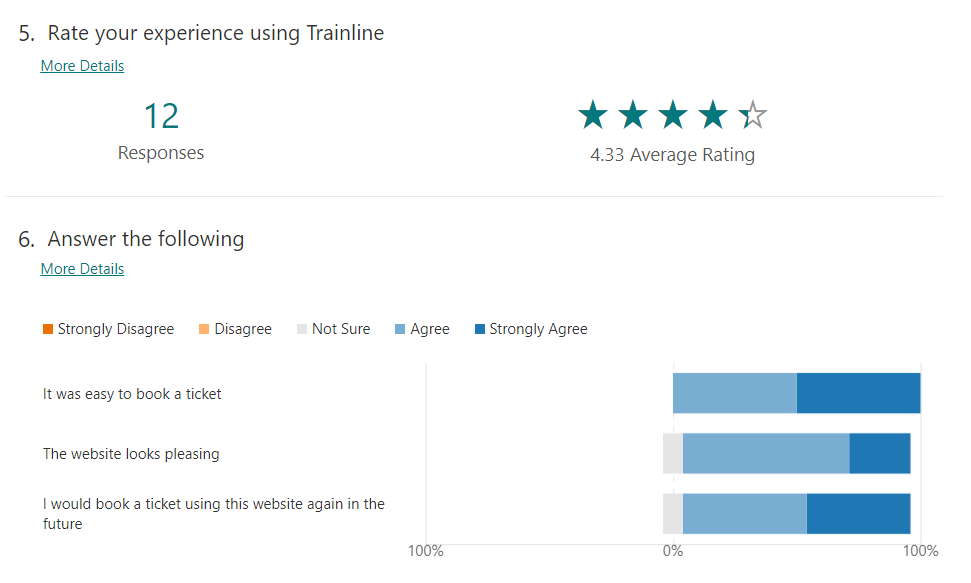
\includegraphics[width=\textwidth]{TrainlineEval.png}
        \caption{A screenshot of \code{Trainline.com}'s ratings from the survey}
        \label{fig:evaltrainline}
    \end{figure}
    
    Using \textit{Microsoft Forms} and \code{Heroku} as mentioned in \cref{sec:deploy}, We asked 12 people with little computer science or web experience, since they would be less biased, to complete a survey created by us. We asked them to use \code{trainline.com} and our chatbot which was hosted publicly for them to access. They were asked to give each system a rating, describe their strengths and weaknesses and more.
    
    \begin{figure}[!ht]
        \centering
        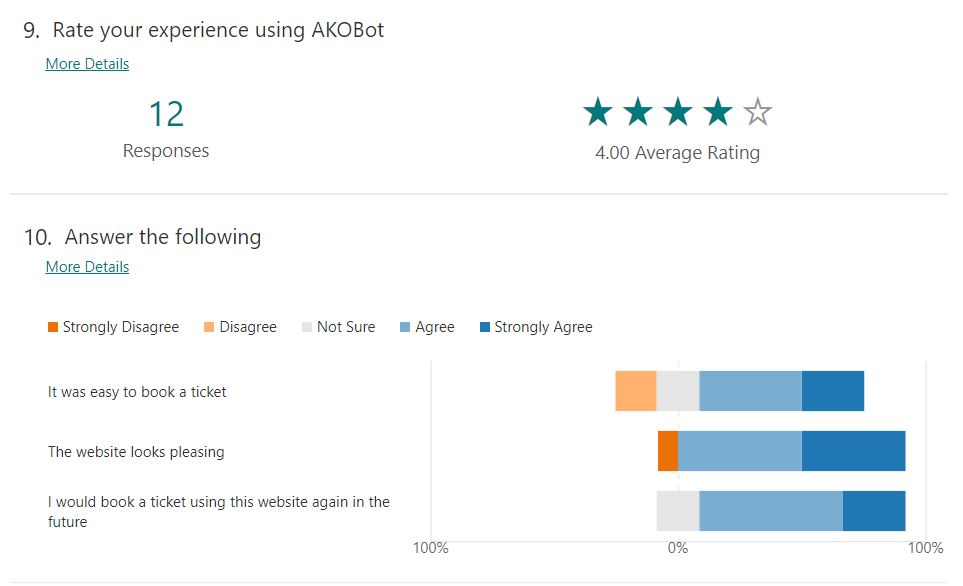
\includegraphics[width=\textwidth]{AkobotEval.png}
        \caption{A screenshot of AKOBot's ratings from the survey}
        \label{fig:evalakobot}
    \end{figure}
    
    As shown in Figures \ref{fig:evaltrainline} and \ref{fig:evalakobot}, AKOBot scored lower than the well-established \code{trainline.com} but it was rated close to it. When the survey was conducted, our chatbot was at incomplete stage. Because of that many surveyed people have pointed out bugs, which were later addressed.
    
    As seen in \cref{fig:akobotPositive}, the majority cited the website's look and simplicity when asked about what they liked about AKOBot. A problem with this evaluation is the fact that we did not wait until we had a completed bug-free system for people to check out, which would mean their first impression is ruined and they would be biased if they were asked to check out the chatbot again after it was already seen before.
    
    
    
    \subsection{Predictive Model}\label{sec:evalmodel}
    The team decided that a model is accurate if it gets the predicted arrival time of a journey within 1 minute of the actual arrival time. As mentioned previously, RF was chosen as the model despite other models which had higher accuracy such as 1NN as seen in \cref{fig:modelEval}.
    
    The reason for choosing RF was simply due to 1NN's nature of not being able to take "y" values, which would have the arrival times which can lead to inconsistency. In addition, we are not able to see the root mean square error (RMSE) in order to supervise the model which makes it somewhat reliable.
    
    The second most accurate model was the MLP-regressor model, which was not chosen because of our inability to check for its \code{R2} and \code{F1} scores. \code{R2} scores are important in order to check for over or under-fitting of the data, so we can not determine how "realistic" the prediction is. \code{F1} scores are also important since it is a slight measure of accuracy by checking against "false-positive" cases, which basically means accurate consistency in our model.
    
    Since RF had the highest accuracy while providing high \code{F1} and consistent {R2} scores compared to other models, which is why we chose RF as the best model for AKOBot.
    

\section{Conclusion}

    \subsection{Future Improvements}
    The chatbot could be considered as good but many components could be heavily improved.
    
    The NLP module could be improved by adding a custom-trained model, where we are able to enter multiple forms of user input in which case we would not have spent so much time in making sure we are able to predict every possible user input.
    
    The predictive model could be improved if we experimented with many more models and finding a way to have models which are stored instead of built at run-time in order to save time. This way, we could have incorporated much more training data into the model including weather data which is a huge factor in determining train delays.
    
    We could add a machine-learning model as the reasoning part of the module instead of having \code{Experta} which is rule-based. This would heavily improve the chatbot into being able to accept a wider variety of user input quickly instead of the current pattern-matching strategy.
    
    \subsection{Summary}
    Creating this chatbot was a difficult task in terms of planning and designing it since we had virtually no experience in most of the components created in this chatbot. It took a long time to learn about each component and effectively come up with ways to deal with the random and unpredictable nature of humans through their input. We found ourselves needing more time in order to fix all the bugs, and add more validation to deal with the inputs.
    
    This however gave the group valuable experience not only in technical terms of NLP, conversation agents and more, but also in terms of dealing with the unpredictable input of humans and long term planning to create such a huge system. This chatbot also was very helpful to especially two of the group members, who have to create a chatbot as their final year projects.
    
    As a group, we think that despite the bugs and missing validation, the chatbot met its goals and is robust in dealing with various user inputs as well looking pleasing and aesthetic that not many chatbots might provide.



\bibliographystyle{agsm}
%\bibliographystyle{apalike}
% you should use your own bibtex file to replace the following example_ref bib file.
\bibliography{refs}
\clearpage
\appendixpage
\begin{appendices}
\section{Screenshots}

\begin{figure}[!ht]
    \centering
    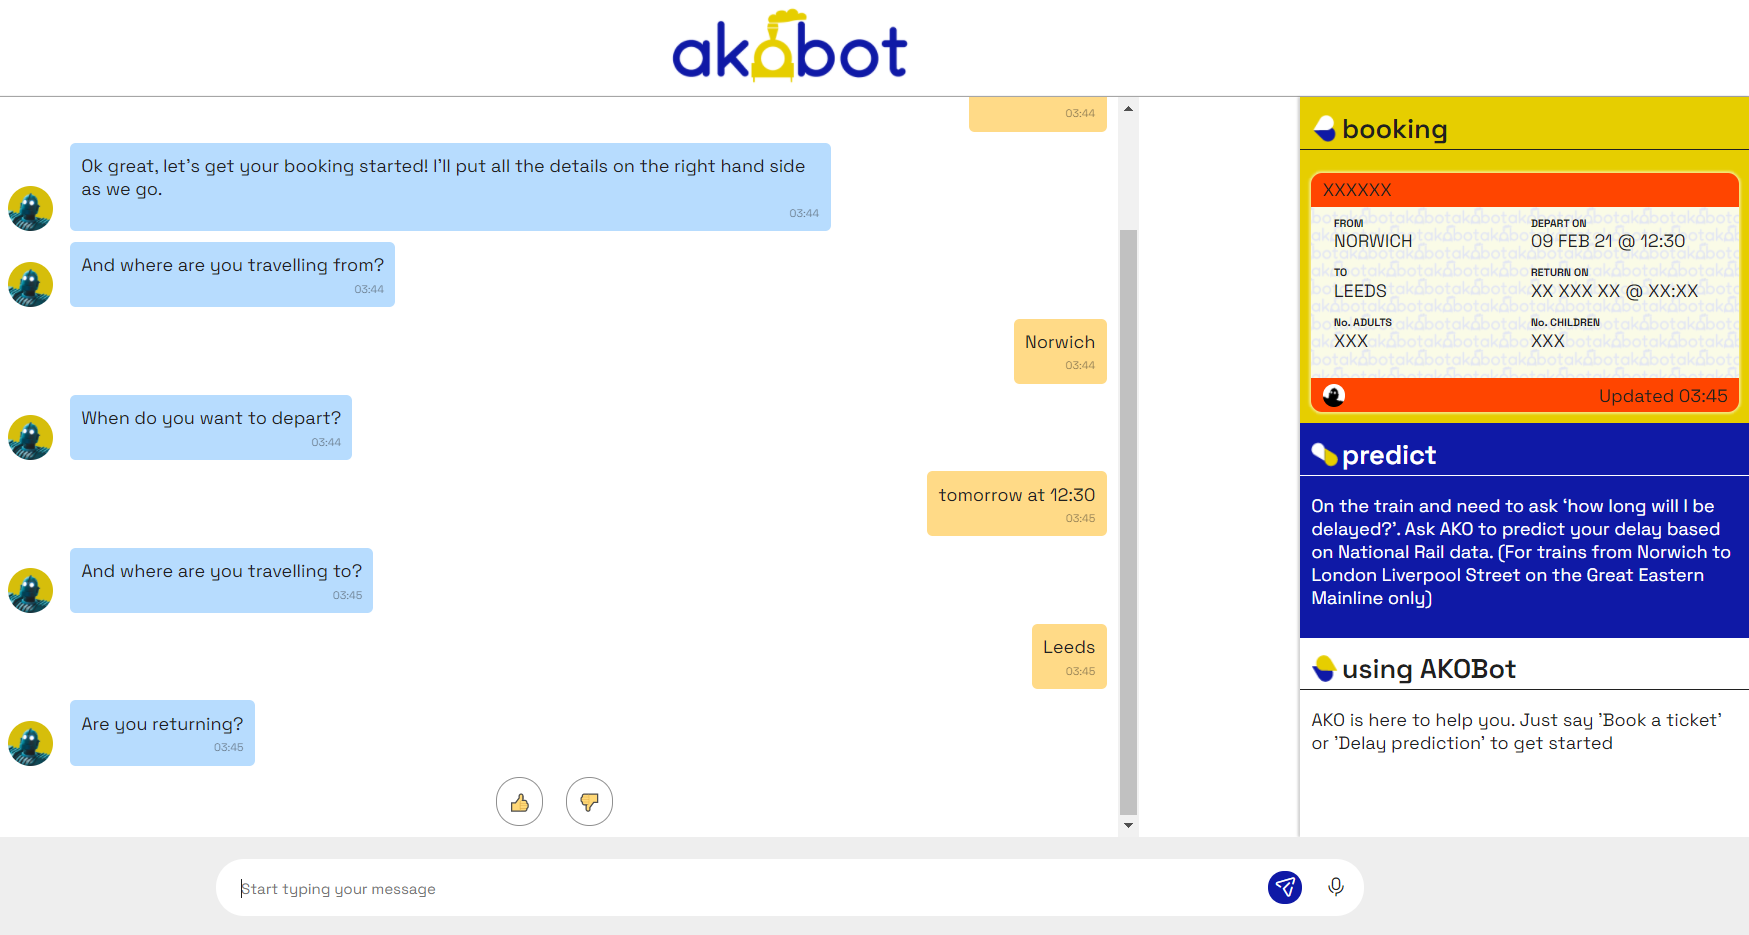
\includegraphics[width=\textwidth]{AkobotSidebar.png}
    \caption{A screenshot of the chatbot with the sidebar shown}
    \label{fig:sidebarAkobot}
\end{figure}

\clearpage
\section{Figures}

\begin{figure}[!ht]
            \centering
            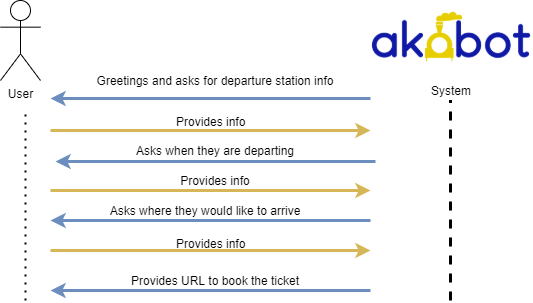
\includegraphics[width=.95\textwidth]{OldBookingFlow.png}
            \caption{An example of a train booking conversation flow}
            \label{fig:OldBookingFlow}
        \end{figure}
        
    \begin{figure}[!ht]
            \centering
            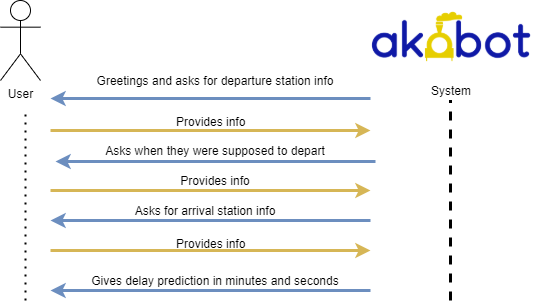
\includegraphics[width=.95\textwidth]{PredictionFlow.png}
            \caption{An example of a delay prediction conversation flow}
            \label{fig:predictFlow}
    \end{figure}
    
    \begin{figure}
        \centering
        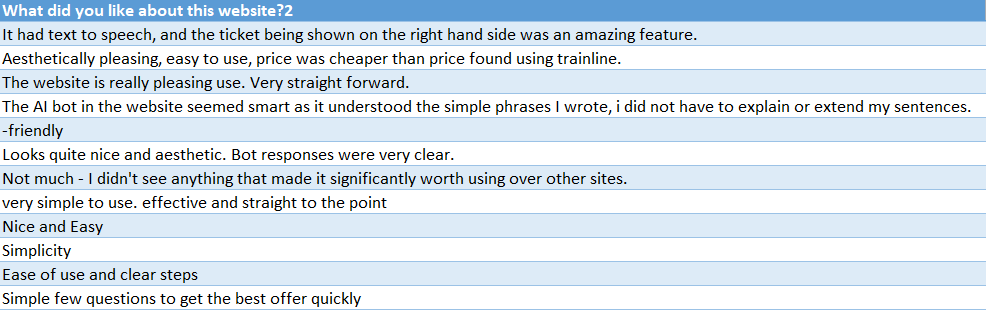
\includegraphics[width=\textwidth]{Akobotlikeval.png}
        \caption{A screenshot of the strengths of AKOBot}
        \label{fig:akobotPositive}
    \end{figure}
    
    \begin{figure}[!ht]
        \centering
        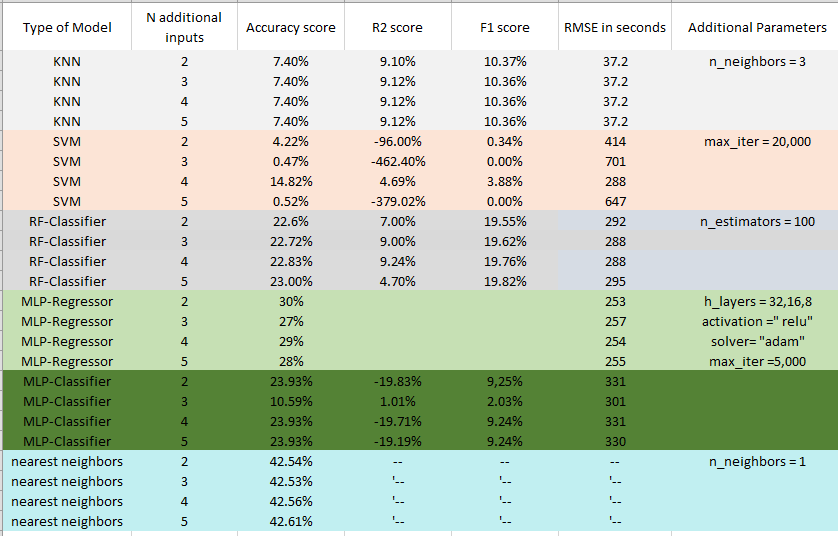
\includegraphics[width=\textwidth]{ModelsEval1.png}
        \caption{A figure showing the results of evaluating prediction models}
        \label{fig:modelEval}
    \end{figure}

\clearpage
\section{Tables}

\begin{table}[!ht]
\centering
\resizebox{\columnwidth}{!}{%
\begin{tabular}{|l|l|l|}
\hline
\textbf{Fact Key}               & \textbf{Value}              & \textbf{Representation}                                                       \\ \hline
\textit{action}                 & "chat" or "book" or "delay" & The type of action which the chatbot is engaged in                   \\ \hline
\textit{complete}               & Boolean                     & Whether the chatbot's task is complete or not                        \\ \hline
\textit{message\_text}          & User message                & The most recent message from the user                                \\ \hline
\textit{depart}                 & Departure station name      & Name of station which user is departing from                         \\ \hline
\textit{arrive}                 & Arrival station name        & Name of station which user is arriving to                            \\ \hline
\textit{departure\_date}        & Departure date/time         & Date and time which user is leaving the departure station            \\ \hline
\textit{extra\_info\_req}       & Boolean                     & Extra information needs to be taken from the user                    \\ \hline
\textit{extra\_info\_requested} & Boolean                     & Extra information question has been asked to the user                \\ \hline
\textit{final\_message\_sent}   & Chatbot message             & The chatbot's ending message is sent after completing ticket booking \\ \hline
\textit{can\_produce\_ending}   & Boolean                     & Whether or not the chatbot can end the conversation                  \\ \hline
\textit{departure\_delay}       & Time in seconds             & Number of seconds the train is delayed by                            \\ \hline
\textit{delay\_time\_received}  & Boolean                     & Whether or not the delay timing from the user has been received      \\ \hline
\textit{no\_adults*}            & Integer                     & Number of adults for ticket booking                                  \\ \hline
\textit{no\_children*}          & Integer                     & Number of children for ticket booking                                \\ \hline
\textit{returning*}             & Boolean                     & Whether or not the user wants a return ticket                        \\ \hline
\textit{return\_date*}          & Return date/time            & Date and time which user is returning at                             \\ \hline
\end{tabular}%
}
\caption{The final table of facts used in the system
Note: Those with "*" are facts which were added during the implementation stage}
\label{tab:REFacts}
\end{table}


\end{appendices}

\end{document}
